%-----------------------Homework------------------------------------
%-------------------Arman Shokrollahi---------------------------------
%---------------------Introduction to Electrical and Electronic Engineering-------------------------------

\documentclass[a4 paper]{article}
% Set target color model to RGB
\usepackage[inner=1.5cm,outer=1.5cm,top=2.5cm,bottom=2.5cm]{geometry}
\usepackage{setspace}
\usepackage[rgb]{xcolor}
\usepackage{verbatim}
\usepackage{amsgen,amsmath,amstext,amsbsy,amsopn,tikz,amssymb,tkz-linknodes}
\usepackage{fancyhdr}
\usepackage[colorlinks=true, urlcolor=blue,  linkcolor=blue, citecolor=blue]{hyperref}
\usepackage[colorinlistoftodos]{todonotes}
\usepackage{rotating}
\usepackage{multirow}
\usepackage{graphicx}
\usepackage{color}
\newcommand{\blue}[1]{\textcolor{blue}{#1}}
\newcommand{\red}[1]{\textcolor{red}{#1}}
\newcommand{\green}[1]{\textcolor{green}{#1}}
\newcommand{\yellow}[1]{\textcolor{yellow}{#1}}
\newcommand{\orange}[1]{\textcolor{orange}{#1}}
\newcommand{\violet}[1]{\textcolor{violet}{#1}}

%\usetikzlibrary{through,backgrounds}
\hypersetup{%
pdfauthor={Nan Meng},%
pdftitle={Notes},%
pdfkeywords={Tikz,latex,bootstrap,uncertaintes},%
pdfcreator={PDFLaTeX},%
pdfproducer={PDFLaTeX},%
}
%\usetikzlibrary{shadows}
\usepackage[francais]{babel}
\usepackage{booktabs}
\newcommand{\ra}[1]{\renewcommand{\arraystretch}{#1}}

      \newtheorem{thm}{Theorem}[section]
      \newtheorem{prop}[thm]{Proposition}
      \newtheorem{lem}[thm]{Lemma}
      \newtheorem{cor}[thm]{Corollary}
      \newtheorem{defn}[thm]{Definition}
      \newtheorem{rem}[thm]{Remark}
      \numberwithin{equation}{section}

\newcommand{\homework}[6]{
   \pagestyle{myheadings}
   \thispagestyle{plain}
   \newpage
   \setcounter{page}{1}
   \noindent
   \begin{center}
   \framebox{
      \vbox{\vspace{2mm}
    \hbox to 6.28in { {\bf ENGG1203:~Introduction to Electrical and Electronic Engineering \hfill} }
       \vspace{6mm}
       \hbox to 6.28in { {\Large \hfill #1 (#2)  \hfill} }
       \vspace{6mm}
       \hbox to 6.28in { {\it Instructor: #3 \hfill TA: #5} }
       %\hbox to 6.28in { {\it TA: #4  \hfill #6}}
      \vspace{2mm}}
   }
   \end{center}
   \markboth{#5 -- #1}{#5 -- #1}
   \vspace*{4mm}
}

\newcommand{\bbF}{\mathbb{F}}
\newcommand{\bbX}{\mathbb{X}}
\newcommand{\bI}{\mathbf{I}}
\newcommand{\bX}{\mathbf{X}}
\newcommand{\bY}{\mathbf{Y}}
\newcommand{\bepsilon}{\boldsymbol{\epsilon}}
\newcommand{\balpha}{\boldsymbol{\alpha}}
\newcommand{\bbeta}{\boldsymbol{\beta}}
\newcommand{\0}{\mathbf{0}}

\begin{document}
\homework{\bf Circuits}{ENGG1203}{Edmund Y.Lam}{}{Nan Meng}{}

% {\begin{tikzpicture}[outline/.style={draw=#1,thick,fill=#1!50}]
% \node [outline=red] at (0,1) {\bf Problem 1};
% \end{tikzpicture}}

\section{Basics}

We use a simple model as a starting point to discuss electronic circuits, which is shown on Figure 1.

\begin{figure}[!ht]
  \caption{Fundamental circuit model}
  \centering
  \includegraphics[width=0.5\textwidth]{./images/introduction}
\end{figure}

\vskip 1em
A basic circuit is made up of a \underline{source} which provides voltage across its terminals, denoted by $V$. 


% --------------------------------------------------------
% --------------------------------------------------------


\subsection{Current}
The current $i$ results from the stream of electric charge around the closed loop shown on Figure 1. The mathematic definition is equal to the amount of charge, $Q$, passing through a cross-section per second and it can be expressed as
\begin{equation}
i = \frac{dQ}{dt} 
\end{equation}
The unit of charge is the Coulomb. One Coulomb is equivalent to $6.24 \times 10^{18}$ electrons.
The unit for current is the ampere, A. One ampere = 1 Coulomb/sec.
 
\subsubsection{Ideal DC current source}
The current source is a device that can provide a certain amount of current to a circuit. The symbol for a DC current source and the i / v characteristic curve of an ideal current source are shown on Figure 2.
\begin{figure}[!ht]
  \caption{Ideal DC current source}
  \centering
  \includegraphics[width=0.09\textwidth]{./images/circuit1/current1}
\end{figure}


% --------------------------------------------------------
% --------------------------------------------------------


\subsection{Voltage}
Moving electrons along a conductor requires some amount of work that must be somehow supplied by an electromotive force provided by a battery or similar device. The electromotive force is the potential difference(voltage) between two points or across a component in circuit. The mathematical definition of voltage is given by
\begin{equation}
v = \frac{dW}{dQ} 
\end{equation}

where work(W) is measured in Joules and charge(Q) in Coulombs.
Basically, the voltage is measured in volts(V) and $1 volt = 1 \frac{Joule}{Coulomb} = 1 \frac{Newton \ meter}{Ampere \ second}$

\subsection{Ideal DC voltage sources}
The voltage provided by a voltage source(usually battery) is constant in time and thus it is called DC voltage. In its ideal implementation the battery provides a specific voltage at all times and for all loads.
The symbols of an ideal DC voltage source are shown as follows:

\begin{figure}[!ht]
  \caption{Ideal DC voltage source}
  \centering
  \includegraphics[width=0.3\textwidth]{./images/circuit1/VoltageSource}
\end{figure}



% --------------------------------------------------------
% --------------------------------------------------------

\subsection{Ideal resistor}
The ideal resistor is a passive, linear, two-terminal device whose resistance follows Ohm`s law given by,
\begin{equation}
v = iR,
\end{equation}
which states that the voltage across an element is directly proportional to the current flowing through the element. The constant of proportionality is the resistance R provided by the element. The resistance is measured in Ohms, $\Omega$, and
\begin{equation}
1 \Omega = 1 \frac{V}{A},
\end{equation}
the symbol for a resistor is,

\begin{figure}[!ht]
  \caption{Ideal resistor}
  \centering
  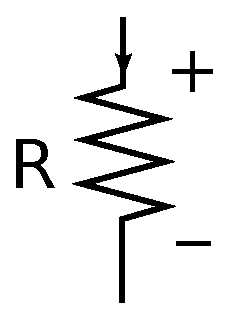
\includegraphics[width=0.1\textwidth]{./images/circuit1/resistor}
\end{figure}



\subsection{Resistor Colour Code}
The coloured painted bands produce a system of identification generally known as a {\bf Resistors Colour Code}.
The resistor colour code markings are always read one band at a time starting from the left to the right, with the larger width tolerance band oriented to the right side indicating its tolerance. By matching the colour of the first band with its associated number in the digit column of the colour chart below the first digit is identified and this represents the first digit of the resistance value.

Again, by matching the colour of the second band with its associated number in the digit column of the colour chart we get the second digit of the resistance value and so on. Then the resistor colour code is read from left to right as illustrated below

\begin{figure}[!ht]
  \caption{Resistor Colour Code}
  \centering
  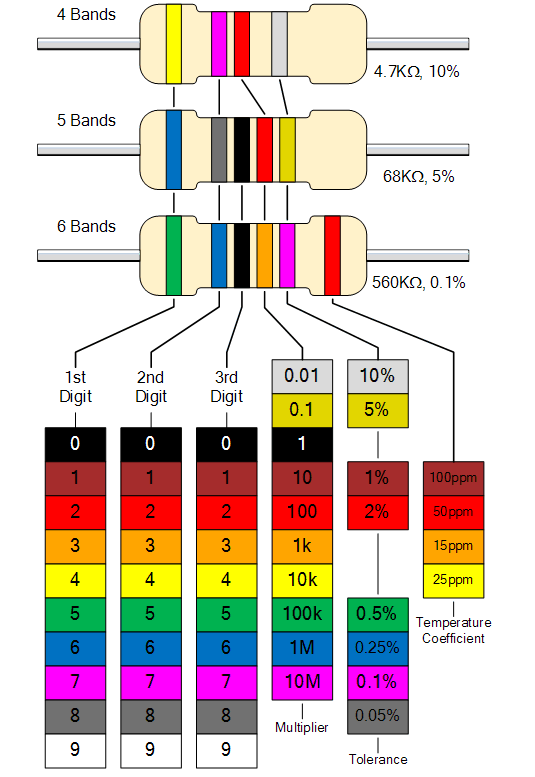
\includegraphics[width=0.5\textwidth]{./images/ColourCode1}
\end{figure}

\vspace{8 mm}

\begin{figure}[!ht]
  \caption{Colour Code Table}
  \centering
  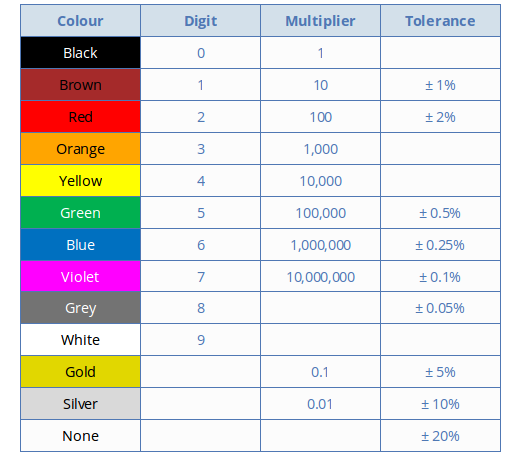
\includegraphics[width=0.5\textwidth]{./images/ColourCode2}
\end{figure}
For example, a resistor has the following colored markings: \newline
\centerline{\yellow{Yellow} \violet{Violet} \red{Red} = \yellow{4} \violet{7} \red{2} = \yellow{4} \violet{7}$\times$ \red{$10_2$} = 4700$\Omega$ or 4k7.
}

\subsection{Power}
When current flows through a resistor, energy is irreversibly lost(or we say dissipated) in overcoming the resistance. THe dissipated power shows up as heat most of the time. The mathematical definition of power is the rate as which energy is delivered that can be expressed as
\begin{equation}
P = \frac{dW}{dt},
\end{equation}
The units for power are $Joules/sec$ or Watts, $W$. ($1 Joules/sec = 1 W$) 
Power can be related to voltage and current by rewriting Eq.(1.5) as, 

\begin{equation}
P = \frac{dW}{dt} = \frac{dW}{dQ}\frac{dQ}{dt}=vi,
\end{equation}

Then substitute Ohm`s law in Eq.(1.6), we will get the power dissipated in a resistor of resistance R is a non-linear function of either $i$ or $v$.

\begin{equation}
P = i^2R \quad or \quad P = \frac{v^2}{R}
\end{equation}
Power rating is a fundamental constraint of resistors and electronic devices in general. The power rating is referred to the maximum power that the device can dissipate without adversely affecting its operation. When the power rating is exceeded the resistor overheats and it is destroyed by burning up. 




% --------------------------------------------------------------
% --------------------------------------------------------------

\section{Kirchhoff’s Laws}
Kirchhoff’s laws also known as Kirchhoff’s Current Law (KCL) and Kirchhoff’s Voltage Law (KVL) are based respectively on the conservation of charge and the conservation of energy and are derived from Maxwell’s equations. They along with Ohm’s law present the fundamental tools for circuit analysis.
\subsection{Kirchhoff’s Current Law}
The current flowing out of any node in a circuit
must be equal to the current flowing into the node. It is expressed mathematically as
\begin{equation}
\sum_{n=1}^{N}i_n=0
\end{equation}

where N is the number of branches that are connected to the node. Consider the node shown on Figure 9. By adopting the sign convention that current flowing ito a node is positive (+) and current flowing out of the node is negative (-), application of KCL gives
\subsection{Kirchhoff’s Voltage Law}
The algebraic sum of voltages around a closed loop is zero. It is expressed mathematically as
\begin{equation}
\sum_{n=1}^{N}v_n=0
\end{equation}

where N is the number of voltages in the loop. The number of voltages is equal to the number of elements encountered as we go around the loop.

\vspace{60 mm}
Next we will solve for the circuit shown on Figure 7

\begin{figure}[ht!]
  \caption{Example resistive circuit}
  \centering
  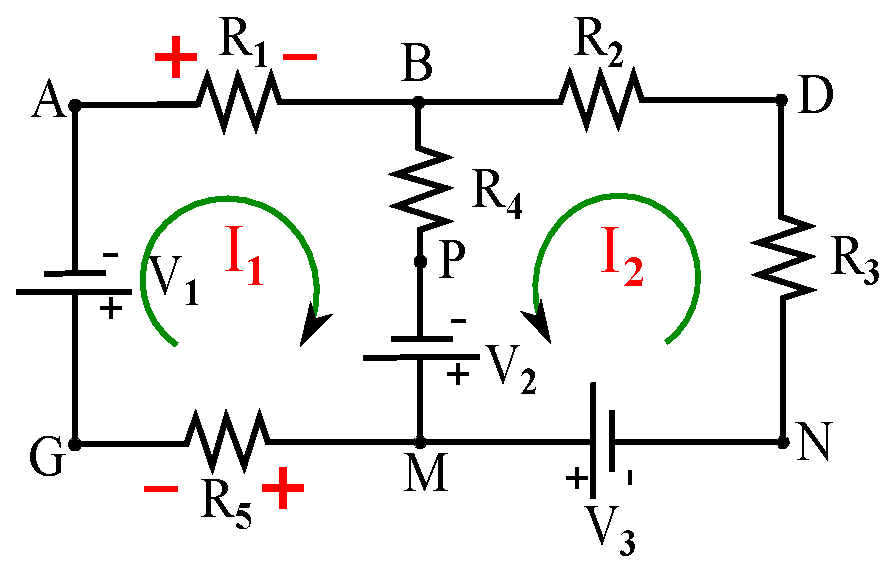
\includegraphics[width=0.5\textwidth]{./images/circuit1/circuit5_1}
\end{figure}
\blue{\centerline{\bf $R_1 = 80\Omega$, $R_2 = 10\Omega$, $R_3 = 20\Omega$, $R_4 = 90\Omega$, $R_5 = 100\Omega$, $V_1 = 12V$, $V_2 = 24V$, $V_3 = 36V$}}

\vspace{8 mm}
Apply Kirchhoff’s laws.

\begin{itemize} \itemsep1pt \parskip0pt \parsep0pt
  \item[$\bullet$] Start with the nodes.
  \begin{enumerate} \itemsep1pt \parskip0pt \parsep0pt
  \item The middle node P is already accounted for since we assigned the current above and below it the same value, I$_1$.  This is just Kirchhoff’s current law which says that the current going into a node is equal to that going out. 
  \item The bottom and top nodes B and M are exactly the same and KCL for them is \newline \newline 
  \centerline{$I - I_1 + I_2 = 0$}
  since at node B current $I$ and $I_2$ flow in the node B and $I_1$ flow out the node B.
  \end{enumerate}
  \item[$\bullet$] Next let's apply KVL to the three loops
  \begin{enumerate} \itemsep1pt \parskip0pt \parsep0pt
    \item {\bf Loop 1($I_1$ loop):} voltage source $V_1$, $V_2$ and resistors $R_1$, $R_4$, $R_5$ \newline\newline
    \centerline{$V_1 + I_1R_1 + (I_1+I_2)R_4 - V_2 + I_1R_5 = 0$}\newline
    \item[] \hspace{56 mm}$\Rightarrow 12 + 80I_1 + 90I_1 + 90I_2 - 24 + 100I_1 = 0$
    \newline
    \item[] \hspace{56 mm}$\Rightarrow 270I_1 + 90I_2 = 12$
    \newline

    \item {\bf Loop 2($I_2$ loop):} voltage source $V_2$, $V_3$ and resistors $R_2$, $R_3$, $R_4$ \newline\newline
    \centerline{$V_3 + I_2R_3 + I_2R_2 + (I_1 + I_2)R_4 -V_2 = 0$}
    \newline
    \item[] \hspace{56 mm}$\Rightarrow 36 + 20I_2 + 10I_2 + 90I_1 + 90I_2- 24 = 0$ \newline
    \item[] \hspace{56 mm}$\Rightarrow 90I_1 + 120I_2 = -12$
    \newline
  
  \end{enumerate}
  \item[$\bullet$] Calculate the required parameters using Ohm`s law and relevant formulas.
  \begin{enumerate} \itemsep1pt \parskip0pt \parsep0pt
    \item[] \centerline{$I_1 = \frac{14}{135}A$}
    \item[] \centerline{$I_2 = -\frac{8}{45}A$}
  \end{enumerate}

\end{itemize}








\section{Voltage divider: Series Connection of Resistors}
The voltage divider circuit is the most convenient means of passively stepping down the voltage from a fixed voltage source. 


\begin{figure}[ht!]
  \centering
  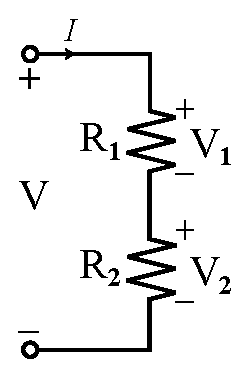
\includegraphics[width=0.15\textwidth]{./images/circuit1/append_end2}
\end{figure}


\begin{itemize} \itemsep1pt \parskip0pt \parsep0pt 
  \item[] \hspace{6.6 cm}{$I=\frac{V}{R_1 + R_2}$}
  \item[] \hspace{6.6 cm}$V_1 = R_1I = \frac{R_1}{R_1 + R_2}V$
  \item[] \hspace{6.6 cm}$V_2 = R_2I = \frac{R_2}{R_1 + R_2}V$
\end{itemize}

By considering a circuit where we are using N resistors connected in series, we can show that the equivalent resistance is the sum of the resistances.

\begin{equation}
R_{eq} = \sum_{n=1}^{N}R_n=R_1+R_2+...+R_N
\end{equation}


\section{Current Divider: Parallel connection of resistors}
The schematic on Figure 8 shows a simple current divider circuit. Here the two resistors $R_1$ and $R_2$ are connected in parallel. Lets determine the current $I_1$ and $I_2$ flowing in the two resistors.

\begin{figure}[ht!]
  \caption{Current Divider}
  \centering
  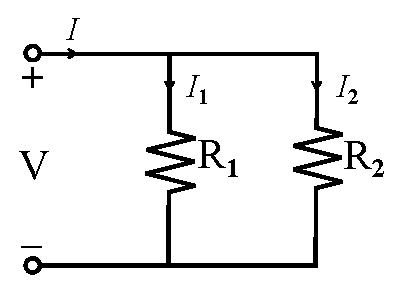
\includegraphics[width=0.3\textwidth]{./images/circuit1/append_end2_2}
\end{figure}
\begin{itemize} \itemsep1pt \parskip0pt \parsep0pt
  \item[] \hspace{6 cm}$V = (R_1 \parallel R_2)I$
  \item[] \hspace{6 cm}$I_1 = \frac{V}{R_1} = \frac{R_1\parallel R_2}{R_1}I = \frac{R_2}{R_1+R_2}I$
  \item[] \hspace{6 cm}$I_2 = \frac{R_1}{R_1 + R_2}I$
\end{itemize}
\vspace{8 mm}

For N resistors connected in parallel the equivalent resistance is 

\begin{equation}
\frac{1}{R_{eq}} = \sum_{n=1}^{N}\frac{1}{R_n}=\frac{1}{R_1}+\frac{1}{R_2}+...+\frac{1}{R_N}
\end{equation}
Note that the equivalent resistance $R_{eq}$ is smaller than the smallest resistance in the parallel arrangement.  

The equivalent conductance of  N resistors connected in parallel is  

\begin{equation}
G_{eq} = \sum_{n=1}^{N}G_n=G_1+G_2+...+G_N
\end{equation}

where $G_n = \frac{1}{R_n}$. The current flowing through resistor $R_n$ is 

\begin{equation}
i_n = i\frac{G_n}{G_{eq}}
\end{equation}

\section{Appendix}
\subsection{Node Method \& Mesh Method}
With the help of Kirchhoff`s laws and Ohm`s law, we can analyze any circuit to determine the currents and voltages. For formal circuit analysis, the challenge is to derive the smallest set of simultaneous equations that completely define the operating characteristics of a circuit.

Therefore, another two methods have been developed, namely node method and mesh method. We will explain the steps to solve the circuit problem shown on Figure 2.

The Node Method.

Note: Voltage is defined as the potential difference between two points. When we talk about the voltage at a certain point, we imply that the measurement is performed between that point and some other point in the circuit.

The node method or node voltage method is based on the application of KCL, KVL and Ohm`s law. The following part list steps used to analysis a circuit with the node method.

\begin{enumerate} \itemsep1pt \parskip0pt \parsep0pt
  \item Label all the circuit parameters and distinguish the unknown parameters from the known ones.
  \item Identify all nodes of the circuit
  \item Choose a reference node(Ground) and assign to it a potential of $0V$. All other voltages in the circuit are measured with respect to the reference node.
  \item Label the voltage at all other nodes.
  \item Assign and label polarities.
  \item Apply KCL at each node and express the branch currents in terms of the node voltages
  \item Solve the resulting simultaneous equations for the node voltages.
  \item Obtain the branch currents by Ohm`s law.
\end{enumerate}







% {\fbox{\it Solution}}

% We want to solve this problem in two ways.

% \underline{First Way}:

% \begin{center}
% \begin{tikzpicture}[thin,fill opacity=0.7]
% \draw [draw=none, fill=red] (90:1.5) circle (2cm);
% \draw [draw=none, fill=green] (-30:1.5) circle (2cm);
% \draw [draw=none, fill=blue] (210:1.5) circle (2cm);
% \begin{scope}
% 	\clip (90:1.5) circle(2cm);
% 	\draw [draw=none, fill=yellow] (-30:1.5) circle (2cm);
% \end{scope} % blue + red = magenta
% \begin{scope}
% 	\clip (210:1.5) circle(2cm);
% 	\draw [draw=none, fill=magenta] (90:1.5) circle (2cm);
% \end{scope}
% \node at (4.1,0) {Circle 2};
% \node at (-4.1,0) {Circle 3};
% \begin{scope} % green + blue = cyan
% 	\clip (-30:1.5) circle(2cm);
% 	\draw [draw=none, fill=cyan] (210:1.5) circle (2cm);
% \end{scope}
% \node at (0,4.1) {Circle 1};
% \begin{scope}
% 	\clip (90:1.5) circle(2cm);
% 	\clip (210:1.5) circle(2cm);
% 	\draw [draw=none, fill=white] (-30:1.5) circle (2cm);	
% \end{scope}
% \node at (1,.5) {$u_0$};
% \node at (0,0) {$u_2$};
% \node at (1.8,-1.1) {$p_1$};
% \node at (-1,.5) {$u_3$};
% \node at (0,-1.2) {$u_1$};
% \node at (0,2) {$p_0$};
% \node at (-2,-1.2) {$p_2$};
% \end{tikzpicture}
% \end{center}
% %
% We know that ${\mathbf v}=({\mathbf{u \; p}})=(u_0u_1u_2u_3 \; p_0p_1p_2)$ has been transmitted. We have
% $r = (1100 \; 001)=(r_0r_1r_2r_3 \; r_4r_5r_6)$ as the received word. We rearrange the above Venn diagram as follows
% %%
% \begin{center}
% \begin{tikzpicture}[thin,fill opacity=0.7]
% \draw [draw=none, fill=red] (90:1.5) circle (2cm);
% \draw [draw=none, fill=green] (-30:1.5) circle (2cm);
% \draw [draw=none, fill=blue] (210:1.5) circle (2cm);
% \begin{scope}
% 	\clip (90:1.5) circle(2cm);
% 	\draw [draw=none, fill=yellow] (-30:1.5) circle (2cm);
% \end{scope} % blue + red = magenta
% \begin{scope}
% 	\clip (210:1.5) circle(2cm);
% 	\draw [draw=none, fill=magenta] (90:1.5) circle (2cm);
% \end{scope}
% \node at (4.1,0) {Circle $2$};
% \node at (-4.1,0) {Circle $3$};
% \begin{scope} % green + blue = cyan
% 	\clip (-30:1.5) circle(2cm);
% 	\draw [draw=none, fill=cyan] (210:1.5) circle (2cm);
% \end{scope}
% \node at (0,4.1) {Circle $1$};
% \begin{scope}
% 	\clip (90:1.5) circle(2cm);
% 	\clip (210:1.5) circle(2cm);
% 	\draw [draw=none, fill=white] (-30:1.5) circle (2cm);	
% \end{scope}
% \node at (1,.5) {$r_0=1$};
% \node at (0,0) {$r_2=0$};
% \node at (1.8,-1.1) {$r_5=0$};
% \node at (-1,.5) {$r_3=0$};
% \node at (0,-1.2) {$r_1=1$};
% \node at (0,2) {$r_4=0$};
% \node at (-2,-1.2) {$r_6=1$};
% \end{tikzpicture}
% \end{center}

% Clearly, Circles $2$ and $3$, in the figure above, have even numbers of $1$'s, but Circle $1$ does not. We conclude that the error cannot be in Circles $2$ and $3$, because their rules are satisfied. So it must be $r_4=0$ that is in error. Thus, $r_4$ must be $1$. Hence, the decoded codeword is
% \begin{equation}
% {\mathbf{\hat{v}}}=(1100 \; 101),
% \label{equ1.1}
% \end{equation}
% from which the decoded data ${\mathbf{\hat{u}}}=(1100)$ may be recovered. \\

% %%
% %%
% %
% \underline{Second Way}:

% We want to solve the problem by some techniques based on generator and parity-check matrices. The parity-check matrix $H$ is helpful in correcting single errors in transmission when
% \begin{enumerate}
%   \item[(i)] $H$ has no column of $0$'s,
%   \item[(ii)] no two columns of $H$ are the same.
% \end{enumerate}
% Consider the following matrix

% $$H=\left(
% \begin{array}{cccccccc}
%   1 & 0 & 1 & 1 & \vdots & 1 & 0 & 0 \\
%   1 & 1 & 0 & 1 & \vdots & 0 & 1 & 0 \\
%   0 & 1 & 1 & 1 & \vdots & 0 & 0 & 1
% \end{array}\right).$$

%  It is easy to check that $H$ satisfies these two conditions and that for the number of rows ($r=3$) in $H$, we have the maximum number of columns possible. If an additional column is added, $H$ will no longer be useful for correcting single errors.\\
% The generator matrix $G$ associated with $H$ is
% $$G=\left(
%   \begin{array}{cccccccc}
%     1 & 0 & 0 & 0 &\vdots & 1 & 1 & 0 \\
%     0 & 1 & 0 & 0 & \vdots& 0 & 1 & 1 \\
%     0 & 0 & 1 & 0 & \vdots& 1 & 0 & 1 \\
%     0 & 0 & 0 & 1 &\vdots & 1 & 1 & 1 \\
%   \end{array}\right).$$
%   Consequently we have a $(7,4)$ group code. The encoding function $E:\mathbb{Z}_2^4 \rightarrow \mathbb{Z}_2^7$ encodes four-bit messages into seven-bit code words. We realize that because $H$ is determined by three parity-check equations (that is, For all $w=w_1w_2w_3w_4\in\mathbb{Z}_2^4$, and $E(w)= wG = w_1w_2w_3w_4w_5w_6w_7 \in \mathbb{Z}_2^7$, now try to find $E(w)=wG$. We get some general equations which are called the {\textit{parity-check equations}}. For more details, see pages 97, 98 of Ryan/Lin), we have now maximized the number of bits we can have in the messages (of course, under our present coding scheme). In addition, the columns of $H$, read from top to bottom, are the binary equivalents of the integers from $1$ to $7$. In general, if we start with $r$ parity-check equations, then the parity-check matrix $H$ can have as many as $2^r-1$ columns and still be used to correct single errors. We denote the transposition of $B$ by $B^{tr}$. Under these circumstances $H=[B\ | \ I_r]$, where $B$ is an $r\times (2^r-1-r)$ matrix, and $G=[I_m\ | \ B^{tr}]$ with $m=2^r-1-r$. The parity-check matrix $H$ associated with a $(2^r-1, 2^r-1-r)$ group code. \\
%   We want to use some terminologies which can be found on pages 103, 104, and 105 of Ryan/Lin. We now have the matrix $H$ for a Hamming $(7,4)$ code. It is easy to check that the coset leader for the syndrome $(100)$ is $(0000 \; 100)$. Why we are talking about  $(100)$? because it is the syndrome corresponding to our received word $r=(1100 \; 001)$; note that
%   $$H \cdot r^{tr}=
%   \left(
%     \begin{array}{c}
%       1 \\
%       0 \\
%       0 \\
%     \end{array}
%   \right).$$
%   Finally, if we assume that $c$ is the transmitted word, then $c=(0000 \; 100)+(1100 \; 001)= (1100 \; 101)\stackrel{\text{\tiny\ref{equ1.1}}}{=} \bf\hat{v}$. \\


%
%
%
%
%
\end{document}
%%------------ Arman Shokrollahi--------------%%
